% ===========================================================================
% chapters/governing_equations.tex — Governing Equations and Finite Volume
%                                     Discretisation
% ===========================================================================

\chapter{Tubular Reactor Model and Spatial Discretisation}\label{ch:governing_eqs}

This chapter develops the mathematical framework that connects the kinetic model of \cref{ch:kinetic_model} to a numerically tractable system. The convection-diffusion-reaction equation governing species transport in a plug flow reactor (PFR) is first derived from mass conservation principles. The partial differential equation is then discretised in space using the finite volume method (FVM), yielding a system of ordinary differential equations suitable for the time integration methods studied in subsequent chapters. Particular emphasis is placed on the conservation properties of FVM and their physical significance for the reactive flow problem.

\section{The Plug Flow Reactor Model}\label{sec:pfr_model}

The reactor is modelled as a one-dimensional tube of length~\(L\) and constant cross-sectional area~\(A\), following the standard axial dispersion model~\cite{Levenspiel1999, Froment2011}. The gaseous reaction mixture flows at superficial velocity~\(u\) along the axial coordinate~\(x \in [0, L]\). The following assumptions reduce the three-dimensional transport problem to a single spatial dimension:

%
\begin{itemize}
  \item Radial concentration and temperature gradients are negligible.
  \item The flow is axially symmetric --- no angular variation.
  \item The overall pressure is approximately constant along the reactor.
  \item The cross-sectional area of the reactor is constant.
\end{itemize}

Under these conditions, the molar concentration~\(C_i(x,t)\) of species~\(i\) is governed by the one-dimensional species transport equation

%
\begin{equation}
  \frac{\partial C_i}{\partial t}
  + u\,\frac{\partial C_i}{\partial x}
  = \Dax\,\frac{\partial^2 C_i}{\partial x^2}
  + \Ri
  \label{eq:species_transport}
\end{equation}
%

where

%
\begin{itemize}
  \item \(C_i\) is the molar concentration of species~\(i\)
        \([\si{\mole\per\metre\cubed}]\),
  \item \(u\) is the superficial gas velocity \([\si{\metre\per\second}]\),
  \item \(\Dax\) is the axial dispersion coefficient
        \([\si{\metre\squared\per\second}]\),
  \item \(\Ri\) is the net volumetric rate of production of
        species~\(i\) \([\si{\mole\per\metre\cubed\per\second}]\), computed
        from the rate expressions developed in
        \cref{ch:kinetic_model}.
\end{itemize}

The four terms in \cref{eq:species_transport} have distinct physical meanings. The first term on the left-hand side, \(\partial C_i / \partial t\), represents the local accumulation of species~\(i\). The second term, \(u\,\partial C_i / \partial x\), describes convective transport --- the bulk gas flow carries species downstream. On the right-hand side, the dispersion term \(\Dax\,\partial^2 C_i / \partial x^2\) accounts for axial spreading caused by turbulent mixing and molecular diffusion. The source term \(R_i\) couples the transport equation to the chemical kinetics of \cref{ch:kinetic_model}.

\subsection{Boundary and Initial Conditions}\label{ssec:boundary_conditions}

At the reactor inlet (\(x = 0\)), a Danckwerts boundary condition~\cite{Danckwerts1953} balances the convective and diffusive fluxes:

%
\begin{equation}
  u\,C_i\big|_{x=0^-}
  = u\,C_i\big|_{x=0^+}
  - \Dax\,\frac{\partial C_i}{\partial x}\bigg|_{x=0^+}
  \label{eq:danckwerts_inlet}
\end{equation}
%

For the idealised PFR, where axial dispersion is small (\(\Dax \to 0\)), this reduces to a Dirichlet condition:
%
\begin{equation}
  C_i(0, t) = \Cin(t)
  \label{eq:dirichlet_inlet}
\end{equation}
%
At the reactor outlet (\(x = L\)), a zero-gradient (Neumann) condition represents fully developed flow with no diffusive flux leaving the domain:
%
\begin{equation}
  \frac{\partial C_i}{\partial x}\bigg|_{x=L} = 0
  \label{eq:neumann_outlet}
\end{equation}
%
The initial condition specifies the concentration distribution at \(t = 0\):
%
\begin{equation}
  C_i(x, 0) = C_{i,0}(x)
  \label{eq:initial_condition}
\end{equation}
%
\subsection{The P\'eclet Number and Convection Dominance}\label{ssec:peclet}

The relative importance of convective and diffusive transport is characterised by the P\'eclet number:
%
\begin{equation}
  \Pe = \frac{u\,L}{\Dax}
  \label{eq:peclet}
\end{equation}
%
which represents the ratio of the convective transport rate to the diffusive transport rate. For tubular reactors the axial dispersion coefficient \(\Dax\) must be estimated from the flow regime. In the laminar regime (\(\Re < 2100\)), the Aris-Taylor analysis~\cite{Taylor1953, Aris1956} gives
%
\begin{equation}
  \Dax = D_{AB} + \frac{u^2\,R^2}{48\,D_{AB}},
  \label{eq:aris_taylor}
\end{equation}
%
where \(D_{AB}\) is the molecular diffusivity and \(R\) the tube radius. For the turbulent and transitional regimes, Fogler~\cite{Fogler2006} (Chapter~14, Figures~14-10 and 14-11, pp.~964--965) summarises experimental correlations giving the dimensionless dispersion number \(\Dax/(u\,d_t)\) as a function of the Reynolds and Schmidt numbers. For typical tubular reactors at high temperature, P\'eclet numbers of order \(10^3\) to \(10^5\) can be inferred from these correlations~\cite{Fogler2006, Levenspiel1999, Froment2011}, indicating strong convection dominance. This has two important consequences.

First, the species concentration profile develops a steep front that propagates downstream with the flow, and diffusion plays only a minor smoothing role.

Second, the choice of numerical scheme for the convective term becomes critical: naive central differencing produces unphysical oscillations when convection dominates, as will be discussed in \cref{ssec:convective_flux}.

In the limiting case \(\Pe \to \infty\), the dispersion term vanishes entirely and \cref{eq:species_transport} reduces to the pure convection-reaction equation of an ideal PFR\@.

\section{Finite Volume Discretisation}\label{sec:fvm}

The finite volume method converts the partial differential \cref{eq:species_transport} into a system of ordinary differential equations by dividing the reactor into discrete control volumes and enforcing mass conservation over each one. The key advantage of FVM is that conservation is guaranteed by construction --- the method is derived directly from the integral form of the conservation law, as explained below.

\subsection{The CSTR Cascade Approximation}\label{ssec:cstr_cascade}

Before systematic spatial discretisation techniques such as FVM became standard in chemical engineering practice, plug flow behaviour was commonly approximated by connecting \(N\) ideally mixed continuous stirred tank reactors (CSTRs) in series~\cite{Kosek2022, Levenspiel1999}. Each tank in the cascade has identical volume \(V\) and is fed at a constant volumetric flow rate \(\dot V\), so that its mean residence time is \(\tau = V/\dot V\). For an inert tracer, the molar balance of species \(A\) in the \(i\)-th tank reads
%
\begin{equation}
  \frac{\mathrm{d}c_{A,i}}{\mathrm{d}t}
  = \frac{1}{\tau}\,\bigl(c_{A,i-1} - c_{A,i}\bigr),
  \qquad i = 1,\,\ldots,\,N,
  \label{eq:cstr_cascade_balance}
\end{equation}
%
with \(c_{A,0}(t)\) prescribing the inlet concentration to the first tank. The hydrodynamic character of this idealised cascade is conventionally analysed through its residence time distribution (RTD), introduced by Danckwerts~\cite{Danckwerts1953}. For a Dirac pulse injected at the inlet, the differential RTD function at the outlet of the cascade is~\cite{Kosek2022, Levenspiel1999}
%
\begin{equation}
  E(t)
  = \frac{t^{N-1}}{(N-1)!}\,
    {\left(\frac{N}{\tau}\right)}^{N}\,
    \exp\!\left(-\frac{N\,t}{\tau}\right),
  \label{eq:rtd_cascade}
\end{equation}
%
which is a Gamma distribution of shape parameter~\(N\). The full derivation proceeds by integrating \cref{eq:cstr_cascade_balance} for a tracer pulse and is given in~\cite{Kosek2022}. For \(N = 1\), \cref{eq:rtd_cascade} reduces to the familiar exponential decay \(E(t) = (1/\tau)\exp(-t/\tau)\) of a single perfectly mixed tank. As \(N\) grows, the distribution narrows into a peak that is centred at \(t = \tau\), and in the limit \(N \to \infty\) it approaches the Dirac delta \(\delta(t - \tau)\), corresponding to the complete absence of axial mixing --- that is, ideal plug flow. \cref{fig:rtd_cascade} illustrates this convergence for several values of~\(N\).

\begin{figure}[H]
\centering
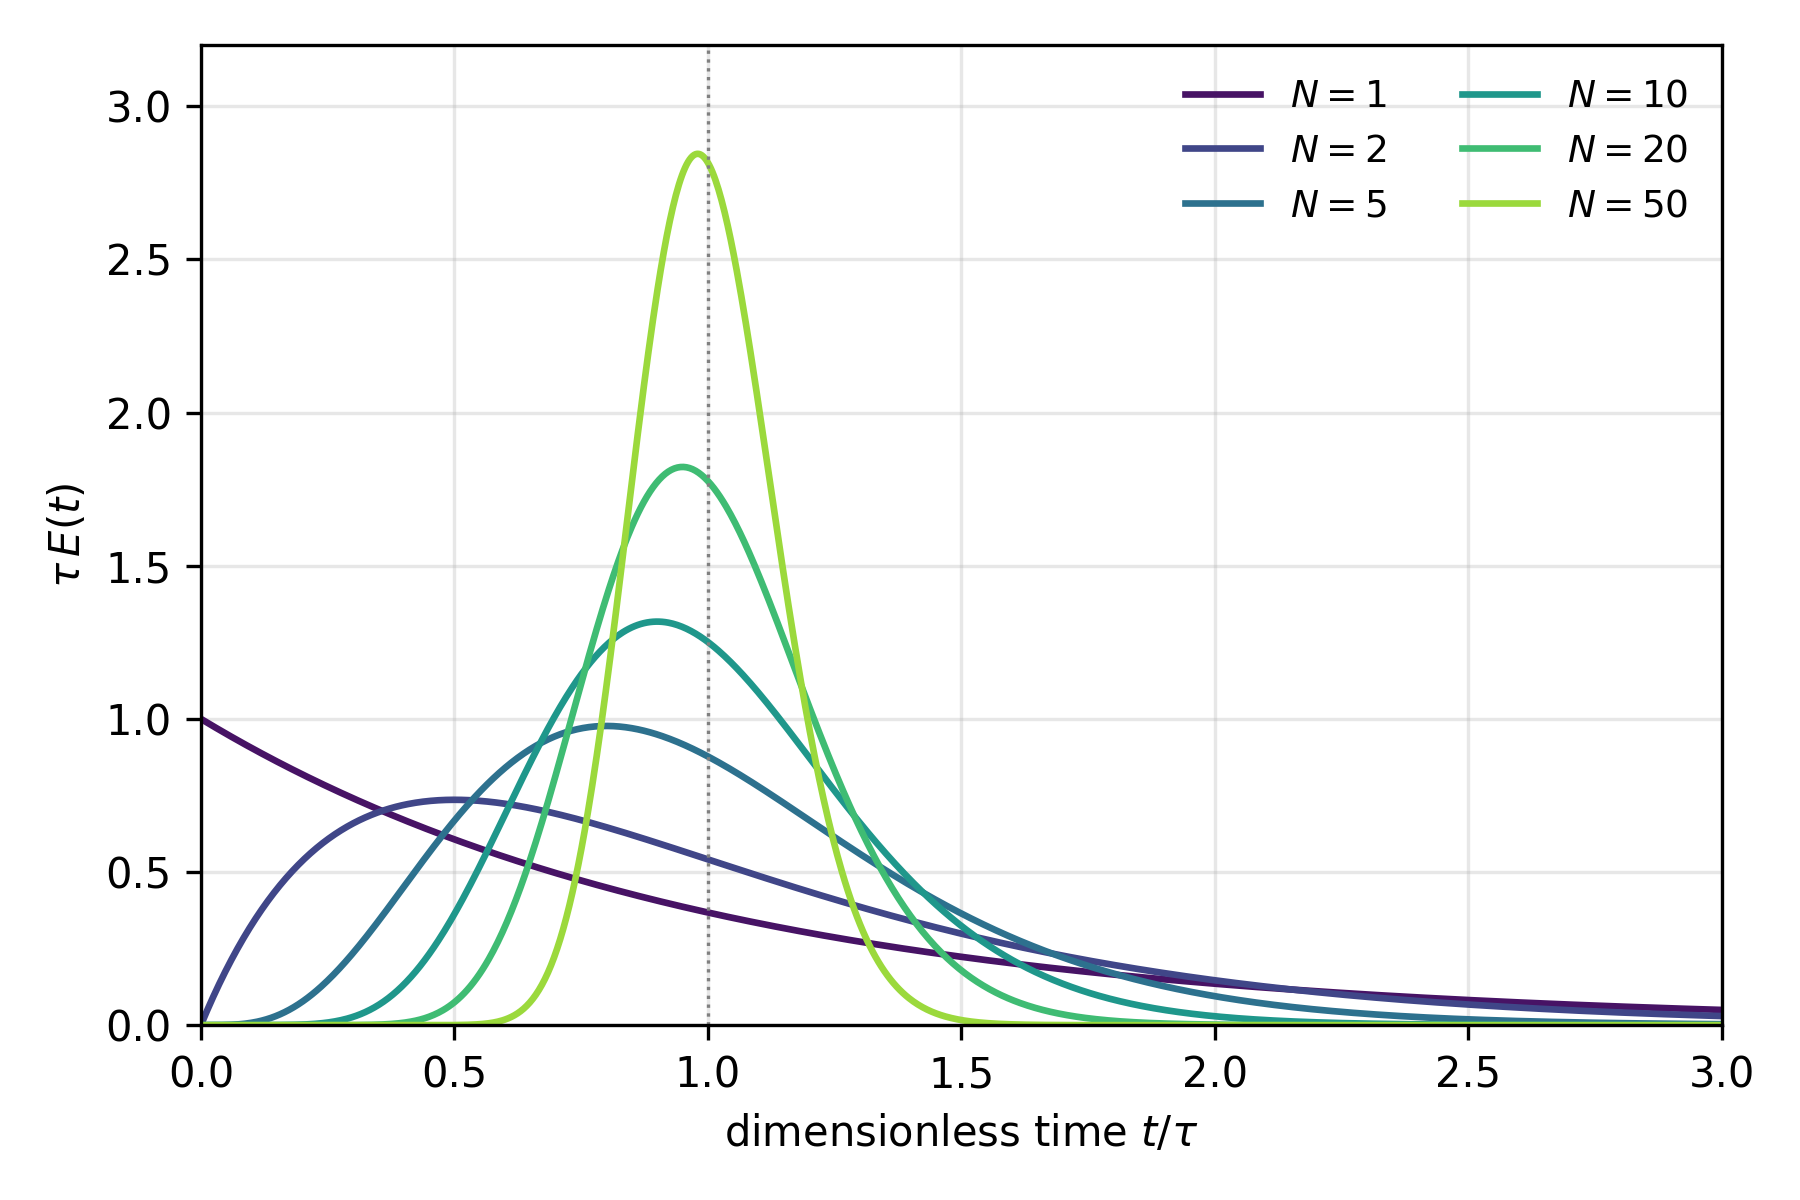
\includegraphics[width=0.68\textwidth]{figures/rtd_cascade.png}
\caption{Differential residence time distribution function \(E(t)\), shown in
the dimensionless form \(\tau\,E(t)\) versus \(t/\tau\), for a cascade of
\(N\) ideally mixed CSTRs. As \(N\) increases, the distribution narrows around
the mean residence time, and in the limit \(N \to \infty\) it converges to the
Dirac delta of an ideal plug flow reactor.}\label{fig:rtd_cascade}
\end{figure}
\FloatBarrier

The finite volume method developed in the remainder of this chapter can be viewed as a formal generalisation of this older engineering intuition. In FVM the reactor domain is partitioned into \(N\) computational cells, each of which carries a single cell-averaged concentration --- effectively the assumption that the field is well mixed within the cell. 

The first-order upwind flux introduced in \cref{ssec:convective_flux} mirrors the cascade construction exactly: the convective flux leaving cell~\(j\) is evaluated using the concentration \emph{inside} that cell, just as the outlet stream of a CSTR carries its own well-mixed tank concentration to the next reactor in the series. Mesh refinement, i.e.\ increasing the number of cells, is the spatial counterpart of adding more tanks to the cascade, and the limit \(N \to \infty\) recovers ideal plug flow in both formulations. 

The cascade picture thus provides a direct physical interpretation of why an ostensibly piecewise-constant discretisation is a sensible approximation for a convection-dominated tubular reactor, and it motivates the systematic conservative derivation of the FVM equations that follows.

\subsection{The Integral Conservation Law}\label{ssec:conservation_law}

The species transport \cref{eq:species_transport} is the differential form of a more fundamental statement: the integral conservation law~\cite{LeVeque2002}. For any \emph{spatial} interval \([a,\,b]\) along the reactor axis, mass conservation of species~\(i\) requires
%
\begin{equation}
  \frac{\mathrm{d}}{\mathrm{d}t}
  \int_a^b C_i\,\mathrm{d}x
  = F_i\big|_{x=a} - F_i\big|_{x=b}
  + \int_a^b R_i\,\mathrm{d}x
  \label{eq:integral_conservation}
\end{equation}
%
where \(F_i = u\,C_i - \Dax\,\partial C_i / \partial x\) is the total (convective plus diffusive) flux of species~\(i\) in the positive \(x\)-direction. In other words: the rate of change of the total amount of species~\(i\) between \(a\) and~\(b\) equals the flux entering through the left face minus the flux leaving through the right face, plus the amount produced by chemical reactions within the interval. 

This is a direct expression of mass conservation. Unlike the spatial form~\eqref{eq:species_transport}, which requires the concentration field to be sufficiently smooth, the integral form~\eqref{eq:integral_conservation} remains valid even at discontinuities such as sharp concentration fronts that are common in convection-dominated flows~\cite{LeVeque2002}. 

The finite volume method, as described by Versteeg and Malalasekera~\cite{Versteeg2007} and LeVeque~\cite{LeVeque2002}, discretizes the integral form~\eqref{eq:integral_conservation} directly. Each computational cell occupying interval \([x_{j-1/2},\, x_{j+1/2}]\) is itself a control volume, and the discrete equation for that cell is a conservation statement.

\newpage
A crucial consequence is the \emph{telescoping property}: the flux leaving cell~\(j\) through face~\(j + \tfrac{1}{2}\) is identical to the flux entering cell~\(j{+}1\) through the same face. When the discrete equations for all cells are summed, the internal fluxes cancel exactly, and only the boundary fluxes at \(x = 0\) and \(x = L\) remain. 

This means that the total amount of species in the reactor can change only through the inlet and outlet boundaries or through chemical reaction --- the discretisation itself neither creates nor destroys mass. For the plug flow reactor, this property has a direct physical interpretation: every mole of a species that leaves one control volume enters the next. 

The stoichiometric relationships established by the kinetic model in \cref{ch:kinetic_model} are preserved at the discrete level. Methods that start from the differential form, such as the finite difference method, do not automatically guarantee this cell-by-cell balance and may introduce small but systematic mass conservation errors over long integration times.

\subsection{Domain Decomposition into Control Volumes}\label{ssec:control_volumes}

The reactor domain \([0, L]\) is divided into \(N\) non-overlapping control volumes (cells). Cell~\(j\) occupies the interval \([x_{j-1/2},\, x_{j+1/2}]\) with cell centre~\(x_j\) and width \(\Delta x_j = x_{j+1/2} - x_{j-1/2}\). For a uniform grid, \(\Delta x = L / N\) and \(x_j = (j - \tfrac{1}{2})\,\Delta x\).

%
\begin{figure}[H]
\centering
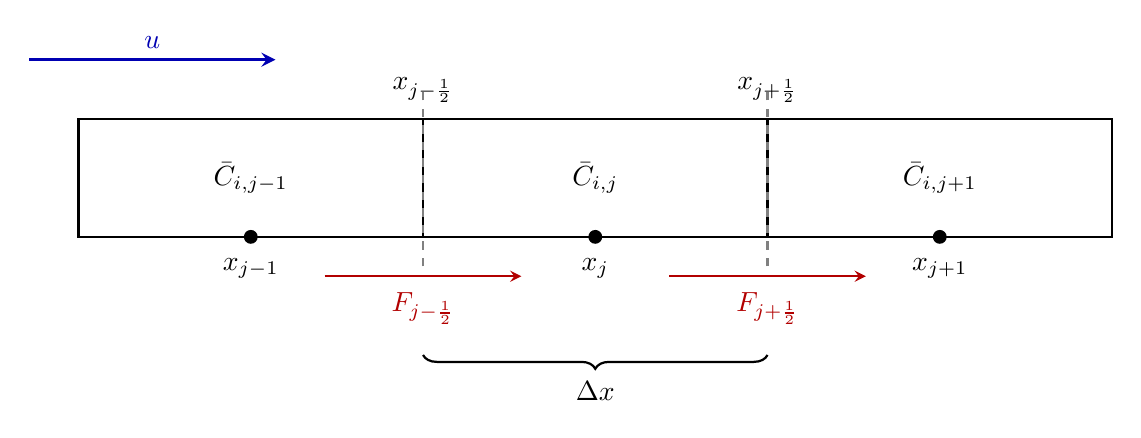
\begin{tikzpicture}[>=stealth, thick, scale=1.25, every node/.style={scale=1.0}]
  % Flow arrow
  \draw[->, very thick, blue!70!black] (-0.5, 1.8) -- (2.0, 1.8)
    node[midway, above] {\(u\)};
  % Cells
  \foreach \j/\lab in {0/{j{-}1}, 3.5/{j}, 7/{j{+}1}} {
    \draw (\j, 0) rectangle (\j+3.5, 1.2);
    \node at (\j+1.75, 0.6) {\(\bar{C}_{i,\lab}\)};
  }
  % Cell centres
  \foreach \j/\lab in {1.75/{j{-}1}, 5.25/{j}, 8.75/{j{+}1}} {
    \fill (\j, 0) circle (2pt);
    \node[below=4pt] at (\j, 0) {\(x_{\lab}\)};
  }
  % Face labels
  \foreach \j/\lab in {3.5/{j{-}\frac{1}{2}}, 7/{j{+}\frac{1}{2}}} {
    \draw[dashed, gray] (\j, -0.3) -- (\j, 1.5);
    \node[above=2pt] at (\j, 1.2) {\(x_{\lab}\)};
  }
  % Flux arrows (below cells to avoid overlap)
  \draw[->, red!70!black, thick] (2.5, -0.4) -- (4.5, -0.4)
    node[midway, below=2pt] {\(F_{j-\frac{1}{2}}\)};
  \draw[->, red!70!black, thick] (6.0, -0.4) -- (8.0, -0.4)
    node[midway, below=2pt] {\(F_{j+\frac{1}{2}}\)};
  % Delta x brace
  \draw[decorate, decoration={brace, amplitude=5pt, mirror}]
    (3.5, -1.2) -- (7, -1.2)
    node[midway, below=6pt] {\(\Delta x\)};
\end{tikzpicture}

\caption{One-dimensional uniform control volume mesh. Cell~\(j\) is bounded by
faces at \(x_{j-1/2}\) and \(x_{j+1/2}\). The cell-averaged concentration
\(\bar{C}_{i,j}\) is stored at the cell centre~\(x_j\). Fluxes \(F\) are
evaluated at each face.}\label{fig:control_volume}
\end{figure}

The unknown quantity in each cell is the cell-averaged concentration:

%
\begin{equation}
  \bar{C}_{i,j}(t)
  = \frac{1}{\Delta x}
    \int_{x_{j-1/2}}^{x_{j+1/2}} C_i(x,t)\,\mathrm{d}x
  \label{eq:cell_average}
\end{equation}
%

\subsection{Integration Over a Control Volume}\label{ssec:fvm_integration}

Integrating \cref{eq:species_transport} over cell~\(j\) gives
%
\begin{equation}
  \int_{x_{j-1/2}}^{x_{j+1/2}}
    \frac{\partial C_i}{\partial t}\,\mathrm{d}x
  + \int_{x_{j-1/2}}^{x_{j+1/2}}
    \frac{\partial\,(u\,C_i)}{\partial x}\,\mathrm{d}x
  = \int_{x_{j-1/2}}^{x_{j+1/2}}
    \Dax\,\frac{\partial^2 C_i}{\partial x^2}\,\mathrm{d}x
  + \int_{x_{j-1/2}}^{x_{j+1/2}} R_i\,\mathrm{d}x
  \label{eq:fvm_integral}
\end{equation}

Applying the fundamental theorem of calculus to the convective and diffusive integrals converts them from volume integrals to surface (face) evaluations:
%
\begin{equation}
  \Delta x\,\frac{\mathrm{d}\bar{C}_{i,j}}{\mathrm{d}t}
  + {\Bigl[u\,C_i\Bigr]}_{x_{j-1/2}}^{x_{j+1/2}}
  = {\biggl[\Dax\,
    \frac{\partial C_i}{\partial x}\biggr]}_{x_{j-1/2}}^{x_{j+1/2}}
  + \Delta x\,\bar{R}_{i,j}
  \label{eq:fvm_semidiscrete_raw}
\end{equation}

The convective and diffusive contributions at each face are collected into fluxes. The convective flux at face \(j + \tfrac{1}{2}\) is
%
\begin{equation}
  F^{\mathrm{c}}_{j+1/2} = u\,C_i\big|_{x_{j+1/2}}
  \label{eq:convective_flux}
\end{equation}
%
and the diffusive flux is
%
\begin{equation}
  F^{\mathrm{d}}_{j+1/2}
  = -\Dax\,
    \frac{\partial C_i}{\partial x}\bigg|_{x_{j+1/2}}
  \label{eq:diffusive_flux}
\end{equation}

Dividing \cref{eq:fvm_semidiscrete_raw} by \(\Delta x\), the semi-discrete equation for cell~\(j\) becomes
%
\begin{equation}
  \frac{\mathrm{d}\bar{C}_{i,j}}{\mathrm{d}t}
  = -\,\frac{F^{\mathrm{c}}_{j+1/2} - F^{\mathrm{c}}_{j-1/2}}{\Delta x}
    -\,\frac{F^{\mathrm{d}}_{j+1/2} - F^{\mathrm{d}}_{j-1/2}}{\Delta x}
    + \bar{R}_{i,j}
  \label{eq:fvm_semidiscrete}
\end{equation}
%
This equation is an exact consequence of mass conservation. The rate of change of the average concentration in a cell equals the net flux through its faces plus the volumetric source term. No approximation has been introduced yet --- the numerical approximation enters only when the face values are reconstructed from cell averages.

\subsection{Approximation of the Diffusive Flux}\label{ssec:diffusive_flux}

The diffusive flux at face \(j + \tfrac{1}{2}\) is approximated by a second-order central difference between adjacent cell centres:
%
\begin{equation}
  F^{\mathrm{d}}_{j+1/2}
  = -\Dax\,
    \frac{\bar{C}_{i,j+1} - \bar{C}_{i,j}}{\Delta x}
  \label{eq:diffusive_flux_approx}
\end{equation}
%
Central differencing is the natural and standard choice for the diffusion operator, which is elliptic and self-adjoint. This approximation is second-order accurate in~\(\Delta x\)~\cite{Versteeg2007, LeVeque2002} and unconditionally stable for the diffusive part of the equation.

\subsection{Approximation of the Convective Flux}\label{ssec:convective_flux}

The convective flux requires the concentration at a cell face, which is not directly available from the cell-averaged unknowns and must be interpolated. A central difference interpolation gives:
%
\begin{equation}
  C_{i,j+1/2}^{\,\mathrm{CD}}
  = \frac{\bar{C}_{i,j} + \bar{C}_{i,j+1}}{2}
  \label{eq:central_interp}
\end{equation}
%
However, central differencing is problematic for the convective term. When this interpolation is substituted into the semi-discrete \cref{eq:fvm_semidiscrete} for pure convection (setting \(\Dax = 0\)), the convective contribution for cell~\(j\) becomes \(u\,(\bar{C}_{i,j+1} - \bar{C}_{i,j-1})/(2\,\Delta x)\). The concentration of cell~\(j\) itself does not appear --- the coefficient on the main diagonal of the resulting matrix is zero. Without diagonal coupling, the even-indexed and odd-indexed cells effectively decouple, and the solution can develop an alternating oscillatory pattern --- a \emph{checkerboard instability} --- that satisfies the discrete equations but is physically meaningless. 

When diffusion is present, it contributes \(\Dax / {(\Delta x)}^{2}\) to the main diagonal, which restores stability provided this diffusive contribution outweighs the off-diagonal convective terms. This condition yields the well-known criterion~\cite{Versteeg2007}: the cell P\'eclet number \(\Pe_{\mathrm{cell}} = u\,\Delta x / \Dax\) must not exceed~2. For the convection-dominated systems considered here, where the global P\'eclet number is of order~\(10^3\), this constraint would require impractically fine grids. The first-order upwind scheme~\cite{Patankar1980} resolves this by using the concentration from the cell upstream of the face --- the cell from which the flow arrives:
%
\begin{equation}
  C_{i,j+1/2}^{\,\mathrm{UW}} =
  \begin{cases}
    \bar{C}_{i,j}   & \text{if } u > 0 \\[4pt]
    \bar{C}_{i,j+1} & \text{if } u < 0
  \end{cases}
  \label{eq:upwind}
\end{equation}
%
For the PFR with \(u > 0\) (flow from inlet to outlet), this simplifies to
%
\begin{equation}
  F^{\mathrm{c}}_{j+1/2} = u\,\bar{C}_{i,j}
  \label{eq:upwind_flux}
\end{equation}
%
The physical justification is that in a convection-dominated flow, information propagates in the direction of the flow. The upwind scheme respects this directionality by always drawing the face value from the upstream cell. Substituting~\eqref{eq:upwind_flux} into the semi-discrete equation, the convective contribution for cell~\(j\) becomes \(u\,(\bar{C}_{i,j} - \bar{C}_{i,j-1})/\Delta x\), which places \(-u/\Delta x\) on the main diagonal of the coefficient matrix. Diagonal dominance is thus restored regardless of the cell P\'eclet number, ensuring unconditional stability of the spatial discretisation.

The upwind scheme is first-order accurate in space~\cite{Patankar1980}. A truncation error analysis shows that this introduces a numerical (artificial) diffusion coefficient:
%
\begin{equation}
  D_{\mathrm{num}} = \frac{u\,\Delta x}{2}
  \label{eq:numerical_diffusion}
\end{equation}
%
so that the discrete scheme effectively solves an equation with dispersion coefficient \(\Dax + D_{\mathrm{num}}\). For a sufficiently refined grid, the numerical contribution remains small compared to the physical dispersion, and the grid can always be refined further to reduce it. 

Stability is more important than high-order accuracy for the stiff reactive system under consideration. \cref{fig:fvm_comparison} illustrates the behaviour of the central and upwind schemes on a steady-state convection-diffusion test problem with an analytical solution, solved as part of a homework assignment given by the thesis supervisor. 

When the cell P\'eclet number remains below~2, both schemes approximate the exact profile well. As convection strengthens and \(\Pe_{\mathrm{cell}}\) exceeds~2, the central scheme develops unphysical oscillations while the upwind scheme stays monotone, albeit with visible numerical diffusion that diminishes on a finer grid.

%
\begin{figure}[H]
\centering
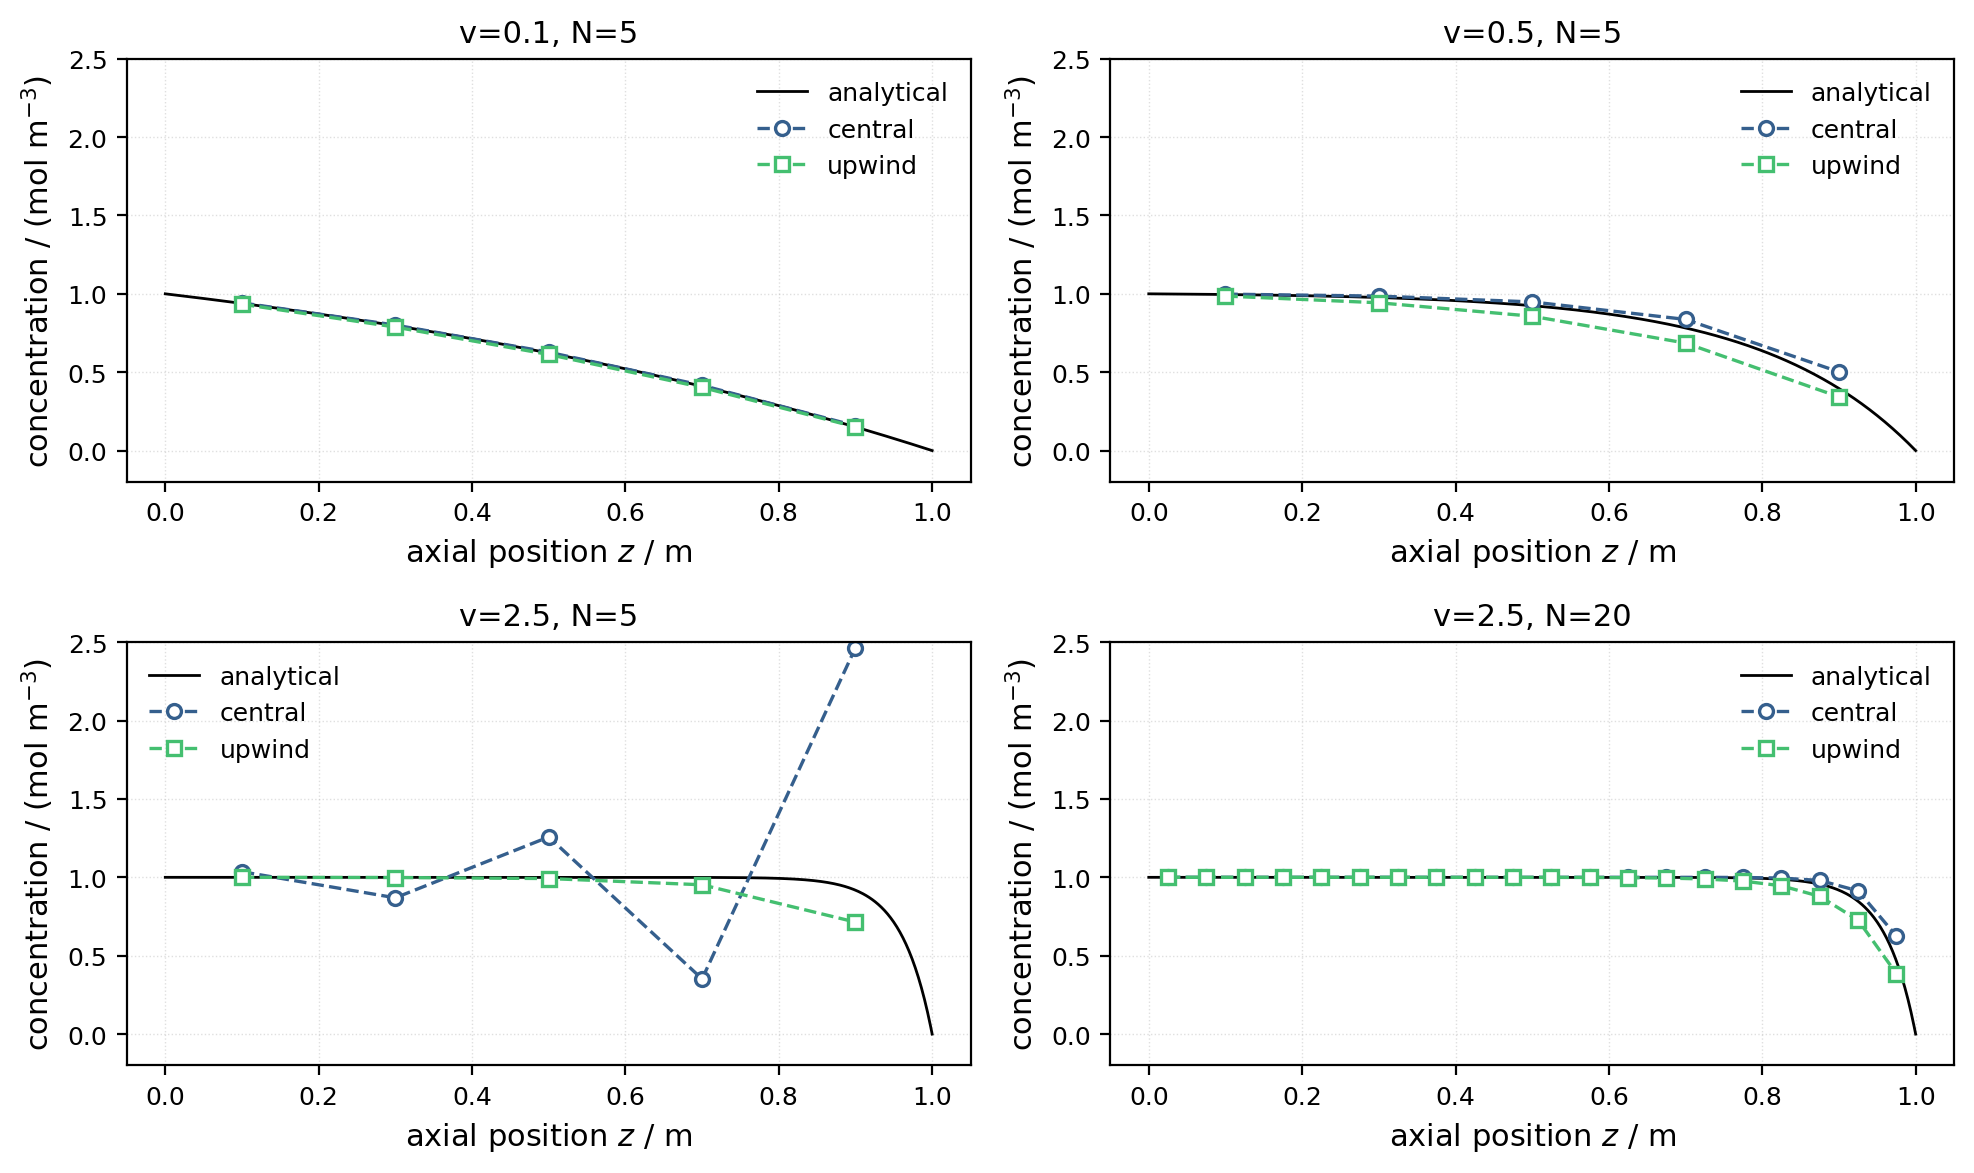
\includegraphics[width=\textwidth]{figures/fvm_comparison.png}
\caption{Central vs.\ upwind FVM schemes against the analytical solution for
steady-state convection-diffusion at four \((v, N)\) settings. As
\(\Pe_{\mathrm{cell}}\) rises, central differencing oscillates while upwind
stays monotone; refinement reduces numerical diffusion. Results from a
homework assignment given by the thesis
supervisor.}\label{fig:fvm_comparison}
\end{figure}
\FloatBarrier

\subsection{The Semi-Discrete System of ODEs}\label{ssec:semidiscrete_ode}

Substituting the upwind convective flux~\eqref{eq:upwind_flux} and the central diffusive flux~\eqref{eq:diffusive_flux_approx} into the semi-discrete \cref{eq:fvm_semidiscrete}, the governing ODE for cell~\(j\) on a uniform grid with \(u > 0\) becomes
%
\begin{equation}
  \frac{\mathrm{d}\bar{C}_{i,j}}{\mathrm{d}t}
  = -\,u\,\frac{\bar{C}_{i,j} - \bar{C}_{i,j-1}}{\Delta x}
    + \Dax\,
      \frac{\bar{C}_{i,j+1} - 2\,\bar{C}_{i,j} + \bar{C}_{i,j-1}}
           {{(\Delta x)}^{2}}
    + R_i{(\bar{\vect{C}}_j, T)}
  \label{eq:semidiscrete_full}
\end{equation}
%
for \(j = 1, 2, \ldots, N\). At the domain boundaries, the flux formulas require concentration values outside the physical domain. These are supplied by \emph{ghost cells}~\cite{LeVeque2002} --- fictitious cells placed at each end of the computational domain. At the inlet, the Dirichlet condition~\eqref{eq:dirichlet_inlet} is enforced by setting the ghost cell value to the inlet concentration, \(\bar{C}_{i,0} = \Cin\). 

The standard upwind formula at face~\(j = \tfrac{1}{2}\) then automatically produces the correct inlet flux \(F^{\mathrm{c}}_{1/2} = u\,\Cin\) without special-casing the first cell. At the outlet, the zero-gradient condition~\eqref{eq:neumann_outlet} is implemented by mirroring the last interior cell: \(\bar{C}_{i,N+1} = \bar{C}_{i,N}\). This ensures that the diffusive flux at the outlet face vanishes and convection simply carries the last cell's concentration out of the domain. 

With these ghost cell definitions, \cref{eq:semidiscrete_full} applies uniformly for all \(j = 1, \ldots, N\) without branching logic at the boundaries. Collecting all cell-averaged concentrations into a single state vector \(\vect{y}(t)\) of dimension \(N_s \times N\), where \(N_s\) is the number of species, the complete system can be written compactly as~\cite{HairerWanner1996}
%
\begin{equation}
  \frac{\mathrm{d}\vect{y}}{\mathrm{d}t} = \vect{f}(\vect{y}, t)
  \label{eq:ode_system}
\end{equation}
%
where the right-hand side \(\vect{f}\) encapsulates the convective fluxes, diffusive fluxes, and reaction source terms. For practical reactor configurations, the total number of equations \(N_s \times N\) can easily reach into the thousands. The system is stiff~\cite{HairerWanner1996} for two reasons. First, the reaction source terms span many orders of magnitude in timescale: widely varying activation energies produce both fast and slow dynamics that must be integrated simultaneously. 

Second, when \(\Dax\) is nonzero and \(\Delta x\) is small, the diffusive eigenvalues scale as \(\Dax / {(\Delta x)}^{2}\), further separating the fastest and slowest timescales. The spatial discretisation thus transforms the original PDE into a stiff ODE system --- precisely the class of problems that motivates the comparison of explicit (forward~Euler), implicit (backward~Euler with Newton iteration), and method-of-lines (BDF via ODEPACK/LSODA) integrators presented in the following chapter.

The state vector is assembled in \emph{cell-grouped ordering}: all species concentrations within each cell are stored consecutively, so that entries \((j-1)\,N_s + 1\) through \(j\,N_s\) correspond to cell~\(j\). This ordering reveals the coupling structure of the right-hand side~\(\vect{f}\). The transport terms (convection and diffusion) couple the \emph{same} species across neighbouring cells --- they link blocks that are \(N_s\) entries apart in the state vector. The reaction terms, by contrast, couple \emph{different} species within the \emph{same} cell --- they act within each block of \(N_s\) consecutive entries.

Implicit time integration methods solve a nonlinear algebraic system at every step via Newton iteration, which in turn requires evaluating and factorising the Jacobian matrix \(\vect{J} = \partial \vect{f} / \partial \vect{y}\). The cell-grouped ordering described above is directly reflected in its sparsity pattern. Because the finite volume stencil connects each cell only to its immediate neighbours, the transport terms contribute a \emph{banded} structure to~\(\vect{J}\) with bandwidth proportional to~\(N_s\). The reaction terms add dense \(N_s \times N_s\) blocks along the main diagonal, since all species within a cell are coupled through the kinetics. The resulting block-banded sparsity enables LU factorisation in \(\mathcal{O}(N_s^{2}\,N)\) operations rather than \(\mathcal{O}((N_s\,N)^{3})\) for a dense matrix~\cite{HairerWanner1996} --- a saving that makes implicit integration of the system computationally feasible.

In summary, the finite volume method has converted the original partial differential \cref{eq:species_transport} into the ODE system~\eqref{eq:ode_system} while preserving the conservation structure of the underlying physics. The telescoping property discussed in \cref{ssec:conservation_law} ensures that the stoichiometric balances of the kinetic model are maintained at the discrete level. The resulting stiff ODE system is directly suitable for the time integration methods studied in the following chapters.
